\documentclass{llncs}

\usepackage{hyperref}

\usepackage[T1]{fontenc} 
\usepackage[utf8]{inputenc}

% \usepackage{amsmath}
% \usepackage{amssymb}
% \usepackage{graphicx}
\usepackage{comment}
% \usepackage{wrapfig}
%\usepackage{url}
% \usepackage{multirow}
\usepackage{color}
% \usepackage{tabularx}  
% \usepackage{booktabs}
% \usepackage{framed}
\usepackage{boxedminipage}
% \usepackage{tikz}
% \usetikzlibrary{arrows,chains,matrix,positioning,scopes}

% \usepackage{enumitem}

% \usepackage{mathpartir}

\usepackage{listings}

%\newcommand{\code}[1]{\lstinline[language={},basicstyle=\lstinfigurestyle]{#1}}
\newcommand{\smcode}[1]{\lstinline[language={},basicstyle=\lstenumstyle]{#1}}
\newcommand{\lstinlinestyle}{\fontfamily{pcr}\fontsize{9pt}{11pt}\selectfont}
\newcommand{\lstfigurestyle}{\fontfamily{pcr}\fontsize{8pt}{10pt}\selectfont}
\newcommand{\lstenumstyle}{\fontfamily{pcr}\fontsize{9pt}{11pt}\selectfont}

%\lstset{backgroundcolor=\color{lightgray}}
\lstset{rulecolor=\color{lightgray}}
\lstset{basicstyle = \lstfigurestyle}
\lstset{tabsize = 2}
\lstset{numberbychapter=false}
\lstset{frame = single, framerule = 0.05pt}
\lstset{numbers = none, numberstyle = \scriptsize\sffamily}%\textcolor{black}}
\lstset{aboveskip=1.5\smallskipamount, belowskip=\smallskipamount}
\lstset{framexbottommargin=0pt}
\lstset{captionpos = t}
\lstset{escapeinside={/+}{+/}}
\lstset{moredelim=*[is][\underbar]{_}{_}}
\lstset{moredelim=[is][basicstyle]{`}{`}} % to escape non-keyword words
\lstset{showstringspaces=false}

\usepackage{atbegshi,ifthen,tikz}

% change this to customize the appearance of the highlight
\tikzstyle{highlighter} = [
  lightgray,
  line width = \baselineskip,
]

% implementation of the core highlighting logic; do not change!
\newcounter{highlight}[page]
\newcommand{\tikzhighlightanchor}[1]{\ensuremath{\vcenter{\hbox{\tikz[remember picture, overlay]{\coordinate (#1 highlight \arabic{highlight});}}}}}
\newcommand{\bh}[0]{\stepcounter{highlight}\tikzhighlightanchor{begin}}
\newcommand{\eh}[0]{\tikzhighlightanchor{end}}
\AtBeginShipout{\AtBeginShipoutUpperLeft{\ifthenelse{\value{highlight} > 0}{\tikz[remember picture, overlay]{\foreach \stroke in {1,...,\arabic{highlight}} \draw[highlighter] (begin highlight \stroke) -- (end highlight \stroke);}}{}}}

\newcommand{\langname}[1]{#1}

\lstdefinelanguage{SDF} {
	morekeywords={context, free, syntax, start, symbols, lexical, module, imports, exports, avoid, recover, cons, bracket, reject, templates, priorities, left},
	otherkeywords={},
	morecomment=[l]{\%\%},
	sensitive=true,
	mathescape=true
}

\newcommand{\sdfcode}[1]{\lstinline[language=SDF,basicstyle=\lstinlinestyle,breaklines=false]{#1}}
\newcommand{\sdfcodebl}[1]{\lstinline[language=SDF,basicstyle=\lstinlinestyle,breaklines=true]{#1}}
\newcommand{\SDF}{\langname{SDF}}

\lstdefinelanguage{SPT} {
	morekeywords={module, test, parse, succeeds, start, symbol, language},
	otherkeywords={[,]},
	morecomment=[l]{\%\%},
	sensitive=true,
	mathescape=true
}

\newcommand{\sptcode}[1]{\lstinline[language=SDF,basicstyle=\lstinlinestyle,breaklines=false]{#1}}
\newcommand{\sptcodebl}[1]{\lstinline[language=SDF,basicstyle=\lstinlinestyle,breaklines=true]{#1}}
\newcommand{\SPT}{\langname{SPT}}

\lstdefinelanguage{Stratego}{
	morekeywords=[1]{all, bagof, constructors, end, extend, fail, id, imports, in,
	let, module, not, one, overlays, override, prim, rec, rules, script, signature,
	some, sorts, rules, strategies, stratego, test, thread, where, with, if, then,
	else, switch, case, otherwise, depends, on}, 
	alsoletter={-}, 
	otherkeywords={<,<+,+>,?.!,*,>,[,$[,|,]}, 
	%morestring=[b]",
	morecomment=[l]{//},
	morecomment=[n]{(*}{*)},
	morecomment=[n]{/*}{*/},
	literate=
		%{|[}{{\texttt{|$\!\!$[}}}2%
		%{]|}{{\texttt{]$\!\!$|}}}2%
		{->}{$\rightarrow$~}2%
		{=>}{$\Rightarrow$~}2,
	sensitive=true,
	mathescape=false,
	keepspaces=true
}[keywords,comments,strings]

\newcommand{\strcode}[1]{\lstinline[language=Stratego,basicstyle=\lstinlinestyle,breaklines=false]{#1}}
\newcommand{\strcodebl}[1]{\lstinline[language=Stratego,basicstyle=\lstinlinestyle,breaklines=true]{#1}}
\newcommand{\Stratego}{\langname{Stratego}}

\lstdefinelanguage{NaBL} {
  morekeywords={module, namespaces, properties, binding, rules, implicitly, defines, unique, of, in, current, subsequent, scope, scopes, refers, to, enclosing, best, conformant, imports, imported, from, as, into, where, has, otherwise, and, or, by, minimal, distance, filters, disambiguates, else, with, error, surrounding},
  otherkeywords={non-unique,non-transitively},
  morekeywords=[2]{}, %% Namespaces
  morekeywords=[3]{}, %% Properties
  morestring=[b]"
	morecomment=[l]{//},
	morecomment=[n]{/*}{*/},
  literate={...}{$\ldots$}2,
  sensitive=true,
  mathescape=false
}

\newcommand{\nablcode}[1]{\lstinline[language=NaBL,basicstyle=\lstinlinestyle,breaklines=false]{#1}}
\newcommand{\nablcodebl}[1]{\lstinline[language=NaBL,basicstyle=\lstinlinestyle,breaklines=true]{#1}}
\newcommand{\NaBL}{\langname{NaBL}}

\lstdefinelanguage{TS} {
	morekeywords={module, imports,type, rules, definition, of, where, has, else, error, on, and, or,function, functions, defines, relations},
  morestring=[b]",
	morecomment=[l]{//},
	morecomment=[n]{/*}{*/},
  sensitive=true,
  mathescape=false
}

\newcommand{\tscode}[1]{\lstinline[language=TS,basicstyle=\lstinlinestyle,breaklines=false]{#1}}
\newcommand{\tscodebl}[1]{\lstinline[language=TS,basicstyle=\lstinlinestyle,breaklines=true]{#1}}
\newcommand{\TS}{\langname{TS}}

\newcommand{\javacode}[1]{\lstinline[language=Java,basicstyle=\lstinlinestyle,breaklines=false]{#1}}
\newcommand{\javacodebl}[1]{\lstinline[language=Java,basicstyle=\lstinlinestyle,breaklines=true]{#1}}
\newcommand{\Java}{\langname{Java}}
\lstdefinelanguage{DynSem} {
  morekeywords={
    module, imports,
    signature, sorts, constructors, native,
    rules, 
    value, 
    where},
  literate={!=}{$\not\equiv$}1{==}{$\equiv$}1{=>}{$\Rightarrow$}1{->}{$\rightarrow$}1{-->}{$\rightarrow$}1{|-}{$\vdash$}1{|-->}{$\mapsto$}1,
  comment=[l]{\/\/},
  mathescape=true,
  sensitive=true
}

\newcommand{\dynsemcode}[1]{\lstinline[language=DynSem,basicstyle=\lstinlinestyle]{#1}}
\newcommand{\DynSem}{\langname{DynSem}}

\newenvironment{dynsemfragment}{\begin{lstlisting}[language=DynSem]}{
\end{lstlisting}}
\lstdefinelanguage{ATerm} {
  morekeywords={},
  morekeywords=[2]{Variable},
  otherkeywords={non-unique,[,]}, % {+,*,?}, % ,-,>
  literate={...}{$\ldots$}2,
  comment=[l]{\%\%},
  mathescape=true,
  sensitive=true
}

\newcommand{\atermcode}[1]{\lstinline[language=ATerm,basicstyle=\lstinlinestyle]{#1}}

% lstlisting coq style (inspired from a file of Assia Mahboubi)
%
\lstdefinelanguage{Coq}{ 
%
% Anything betweeen $ becomes LaTeX math mode
mathescape=true,
%
% Comments may or not include Latex commands
texcl=false, 
%
% Vernacular commands
morekeywords=[1]{Section, Module, End, Require, Import, Export,
  Variable, Variables, Parameter, Parameters, Axiom, Hypothesis,
  Hypotheses, Notation, Local, Tactic, Reserved, Scope, Open, Close,
  Bind, Delimit, Definition, Let, Ltac, Fixpoint, CoFixpoint, Add,
  Morphism, Relation, Implicit, Arguments, Unset, Contextual,
  Strict, Prenex, Implicits, Inductive, CoInductive, Record,
  Structure, Canonical, Coercion, Context, Class, Global, Instance,
  Program, Infix, Theorem, Lemma, Corollary, Proposition, Fact,
  Remark, Example, Proof, Goal, Save, Qed, Defined, Hint, Resolve,
  Rewrite, View, Search, Show, Print, Printing, All, Eval, Check,
  Projections, inside, outside, Def},
%
% Gallina
morekeywords=[2]{forall, exists, exists2, fun, fix, cofix, struct,
  match, with, end, as, in, return, let, if, is, then, else, for, of,
  nosimpl, when},
%
% Sorts
morekeywords=[3]{Type, Prop, Set, true, false, option},
%
% Various tactics, some are std Coq subsumed by ssr, for the manual purpose
morekeywords=[4]{pose, set, move, case, elim, apply, clear, hnf,
  intro, intros, generalize, rename, pattern, after, destruct,
  induction, using, refine, inversion, injection, rewrite, congr,
  unlock, compute, ring, field, fourier, replace, fold, unfold,
  change, cutrewrite, simpl, have, suff, wlog, suffices, without,
  loss, nat_norm, assert, cut, trivial, revert, bool_congr, nat_congr,
  symmetry, transitivity, auto, split, left, right, autorewrite},
%
% Terminators
morekeywords=[5]{by, done, exact, reflexivity, tauto, romega, omega,
  assumption, solve, contradiction, discriminate},
%
% Control
morekeywords=[6]{do, last, first, try, idtac, repeat},
%
% Comments delimiters, we do turn this off for the manual
morecomment=[s]{(*}{*)},
%
% Spaces are not displayed as a special character
showstringspaces=false,
%
% String delimiters
morestring=[b]",
morestring=[d]�?,
%
% Size of tabulations
tabsize=3,
%
% Enables ASCII chars 128 to 255
extendedchars=false,
%
% Case sensitivity
sensitive=true,
%
% Automatic breaking of long lines
breaklines=false,
%
% Default style fors listings
%basicstyle=\small,
%
% Position of captions is bottom
captionpos=b,
%
% flexible columns
columns=[l]flexible,
%
% Style for (listings') identifiers
identifierstyle={\color{black}},
% Style for declaration keywords
keywordstyle=[1]{\color{eclipse-keywords}},
% Style for gallina keywords
keywordstyle=[2]{\color{eclipse-keywords}},
% Style for sorts keywords
keywordstyle=[3]{\color{eclipse-keywords}},
% Style for tactics keywords
keywordstyle=[4]{\color{eclipse-keywords}},
% Style for terminators keywords
keywordstyle=[5]{\color{eclipse-keywords}},
%Style for iterators
%keywordstyle=[6]{\ttfamily\color{dkpink}},
% Style for strings
%stringstyle=\ttfamily,
% Style for comments
commentstyle={\color{eclipse-comments}},
%
%moredelim=**[is][\ttfamily\color{red}]{/&}{&/},
literate=
    {\\forall}{{\color{dkgreen}{$\forall\;$}}}1
    {\\exists}{{$\exists\;$}}1
    {<-}{{$\leftarrow\;$}}1
    {=>}{{$\Rightarrow\;$}}1
    {==}{{\code{==}\;}}1
    {==>}{{\code{==>}\;}}1
%    {:>}{{\code{:>}\;}}1
    {->}{{$\rightarrow\;$}}1
    {<->}{{$\leftrightarrow\;$}}1
    {<==}{{$\leq\;$}}1
    {\#}{{$^\star$}}1 
    {\\o}{{$\circ\;$}}1 
    {\@}{{$\cdot$}}1 
    {\/\\}{{$\wedge\;$}}1
    {\\\/}{{$\vee\;$}}1
    {++}{{\code{++}}}1
    {~}{{\ }}1
    {\@\@}{{$@$}}1
    {\\mapsto}{{$\mapsto\;$}}1
    {\\hline}{{\rule{\linewidth}{0.5pt}}}1
%
}[keywords,comments,strings]

\newcommand{\coqcode}[1]{\lstinline[language=Coq,basicstyle=\lstinlinestyle]{#1}}

\lstdefinelanguage{PCFM} {
	morekeywords={module, import, include, def, fun, let, letrec, letpar, in, fix,
	ifz, then, else}, morestring=[b]",
	morecomment=[l]{//},
	morecomment=[n]{/*}{*/},
  sensitive=true,
  mathescape=true
}


\newcommand{\pcfmcode}[1]{\lstinline[language=PCFM,basicstyle=\lstinlinestyle,breaklines=false]!#1!}
\newcommand{\pcfmcodefig}[1]{\lstinline[language=PCFM,basicstyle=\lstfigurestyle,breaklines=false]!#1!}
\newcommand{\pcfmcodebl}[1]{\lstinline[language=PCFM,basicstyle=\lstinlinestyle,breaklines=true]!#1!}
\newcommand{\PCFM}{\langname{PCFM}}
\newcommand{\pcfmcodemm}[1]{\lstinline[language=PCFM,basicstyle={\fontfamily{pcr}\fontsize{9pt}{11pt}\selectfont},breaklines=true]!#1!}


\lstdefinelanguage{paplj} {
	morekeywords={program, run, class, this, Num, Bool, let, in},
	otherkeywords={},
	morecomment=[l]{\%\%},
	sensitive=true,
	mathescape=true
}

\newcommand{\papljcode}[1]{\lstinline[language=SDF,basicstyle=\lstinlinestyle,breaklines=false]{#1}}
\newcommand{\papljcodebl}[1]{\lstinline[language=SDF,basicstyle=\lstinlinestyle,breaklines=true]{#1}}
\newcommand{\paplj}{\langname{PAPLJ}}


\renewcommand{\ldots}{..}
\renewcommand{\texttt}[1]{\smcode{#1}}



\definecolor{eclipse-keywords}{rgb}{0.55,0,0.337}
\definecolor{eclipse-strings}{rgb}{0.165,0,1}
\definecolor{eclipse-comments}{rgb}{0.247,0.498,0.373}
\definecolor{eclipse-keywords2}{rgb}{0,0.25,0.5}

\definecolor{RoyalBlue}{cmyk}{1,0.50,0,0}


% \newcounter{rqno}
\newcommand{\rqdef}[1]{\refstepcounter{rqno}\emph{RQ\arabic{rqno}}\label{rq:#1}}
\newcommand{\rqref}[1]{\emph{RQ\ref{rq:#1}}}

\newcommand{\sectionlabel}[1]{\label{sec:#1}}
\newcommand{\figurelabel}[1]{\label{fig:#1}}
\newcommand{\listinglabel}[1]{\label{lst:#1}}
\newcommand{\appendixlabel}[1]{\label{apx:#1}}
\newcommand{\tablelabel}[1]{\label{tbl:#1}}

\newcommand{\sectionref}[1]{\ref{sec:#1}}
\newcommand{\figureref}[1]{\ref{fig:#1}}
\newcommand{\listingref}[1]{\ref{lst:#1}}
\newcommand{\appendixref}[1]{\ref{apx:#1}}
\newcommand{\tableref}[1]{\ref{tbl:#1}}

\newcommand{\Section}[1]{Section~\sectionref{#1}}
\newcommand{\Sections}[1]{Sections~#1}
\newcommand{\Figure}[1]{Fig.~\figureref{#1}}
\newcommand{\Figures}[1]{Figures~#1}
\newcommand{\Listing}[1]{Listing~\listingref{#1}}
\newcommand{\Listings}[1]{Listings~#1}
\newcommand{\Appendix}[1]{Appendix~\appendixref{#1}}
\newcommand{\Appendices}[1]{Appendices~#1}
\newcommand{\Table}[1]{Table~\tableref{#1}}
\newcommand{\Tables}[1]{Tables~#1}

%\newtheorem{lemma}{Lemma}
%\newtheorem{thm}{Theorem}
%\newtheorem{def}{Definition}

\newcommand{\mynote}[2]
     %%{\sorrynotesaredisallowedatthispoint}
     {{\bfseries\sffamily\scriptsize#1~{\small$\blacktriangleright$\textsf{\emph{#2}}$\blacktriangleleft$}}}

\newcommand\TODO[1]{\mynote{TODO}{#1}}

\newcommand{\AP}[1]{\mynote{AP}{#1}}
\newcommand{\EV}[1]{\mynote{EV}{#1}}
\newcommand{\PN}[1]{\mynote{PN}{#1}}
\newcommand{\APT}[1]{\mynote{APT}{#1}}
\newcommand{\GW}[1]{\mynote{GW}{#1}}
\newcommand{\cfg}{\ensuremath{G = (N, \Sigma, P, S)}}
\newcommand{\symbols}{\ensuremath{\left(N \cup \Sigma\right)^*}}
\newcommand{\derive}[1]{\ensuremath{\Rightarrow_{#1}}}
\newcommand{\prule}[2]{\ensuremath{\left(#1,#2\right)}}

\newcommand{\kw}[1]{\text{\lmrcodefig{#1}}}
\newcommand{\sep}[1]{\text{\lmrcode{#1}}}
\newcommand{\w}[1]{\ensuremath{\mathit{#1}}}
\newcommand{\te}[1]{\ensuremath{\mathrm{#1}}}

\newcounter{grammarrule}
\newenvironment{grammar}
{\small
\setcounter{grammarrule}{0}
\begin{math}\begin{array}{rrcl}}
{\end{array}\end{math}}

\newcommand{\sdn}[3]{#1 & \w{#2} & = & #3}
\newcommand{\sdnn}[2]{\sdn{}{#1}{#2}}
\newcommand{\sd}[2]{\stepcounter{grammarrule}\sdn{\pno{\arabic{grammarrule}}}{#1}{#2}}
\newcommand{\mc}[2]{ & #1 &  & \mbox{#2}}

\newcommand{\altf}[1]{\ |\ #1}
\newcommand{\altn}[2]{\\ #1 & & | & #2}
\newcommand{\altnn}[1]{\altn{}{#1}}
\newcommand{\alt}{\stepcounter{grammarrule}\altn{\pno{\arabic{grammarrule}}}}
\newcommand{\ks}[1]{\ensuremath{#1^*}}
\newcommand{\opt}[1]{\ensuremath{#1?}}

\lstdefinestyle{black-white}
       {keywordstyle=[2]\textit}
\lstdefinestyle{colours}{%
  keywordstyle={\color{eclipse-keywords}}, %
  keywordstyle=[2]{\color{eclipse-strings}}, %
  keywordstyle=[3]{\color{eclipse-keywords2}}, %
  stringstyle={\color{eclipse-strings}}, %
  commentstyle={\color{eclipse-comments}\textit}, %
}
%\lstset{style=colours}
% 
% Judgements
\newcommand{\firstdec}[1]{\emph{#1}\medskip}
\newcommand{\firstdecj}[2]{\emph{#1}\hfill\framebox{\framebox{#2}}\medskip}
\newcommand{\dec}[1]{\medskip\emph{#1}\medskip}
\newcommand{\decj}[2]{\medskip\emph{#1}\hfill\framebox{\framebox{#2}}\medskip}
\newcommand{\wfj}[2]{\ensuremath{#1\ \vdash #2}}
\newcommand{\wtsj}[4]{\ensuremath{#1\ \vdash #2#3 #4}}
\newcommand{\wtj}[3]{\wtsj{#1}{#2}{\,:\,}{#3}}
\newcommand{\wfji}[3]{\ensuremath{#2\ \vdash_{#1} #3}}
\newcommand{\wtjsi}[5]{\ensuremath{#2\ \vdash_{#1} #3#4 #5}}
\newcommand{\wtji}[4]{\wtsj{#1}{#2}{#3}{\,:\,}{#4}}
\newcommand{\ioj}[3]{\ensuremath{#1\ \vdash #2 \Downarrow #3}}
\newcommand{\iouj}[4]{\ensuremath{#2\ \vdash_{#1} #3 \Downarrow #4}}
\newcommand{\applyj}[3]{\ensuremath{\applyf{#1}{#2} = #3}}
\newcommand{\applyf}[2]{\ensuremath{#1\!\left(#2\right)}}
\newcommand{\domj}[2]{#2 \not\in \applyf{\mathit{dom}}{#1}}

\newcommand{\proj}[2]{\applyf{\pi_{#2}}{#1}}
\newcommand{\fst}[1]{\proj{#1}{1}}
\newcommand{\snd}[1]{\proj{#1}{2}}
% tuple
\newcommand{\tpl}[1]{\ensuremath{\langle\,#1\,\rangle}}

% rule name
\newcommand{\tg}[1]{{[}\ensuremath{\mathsf{#1}}{]}}

% axiom
\newcommand{\ax}[2]{\ensuremath{%
\begin{array}[b]{c}
#2
\end{array}\hfill
\begin{tabular}[c]{r}\vspace{.5em}{\tg{#1}}
\end{tabular}\medskip
}}

% inference rule
\newcommand{\ir}[3]{\ensuremath{%
\begin{array}[b]{c}
#2
\\ \midrule
#3
\end{array}\hfill
\begin{tabular}[b]{r}\vspace{.5em}\tg{#1}
\end{tabular}\bigskip
}}


\newcommand{\infrule}[3]{\ensuremath{%
\hfill\dfrac{
  \displaystyle #2
}{
  \displaystyle #3
}\hspace*{\fill}\makebox[0pt][r]{(\ensuremath{#1})}
}}
\newcommand{\infruleL}[3]{\ensuremath{%
\makebox[0pt][l]{(\ensuremath{#1})}\hfill\dfrac{
  \displaystyle #2
}{
  \displaystyle #3
}\hfill
}}
\newcommand{\infrulenl}[2]{\ensuremath{%
\hfill\dfrac{
  \displaystyle #1
}{
  \displaystyle #2
}\hfill}}


\newcommand{\labeled}[2]{\ensuremath{%
\hfill\ensuremath{\displaystyle #2}\hfill\makebox[0pt][r]{(\ensuremath{#1})}
}}
\newcommand{\labeledL}[2]{\ensuremath{%
\makebox[0pt][r]{(\ensuremath{#1})}\hfill\ensuremath{\displaystyle #2}\hfill
}}

\newcommand{\display}[1]{
\bigskip #1 \bigskip
}

% axiom as inference rule
\newcommand{\axr}[2]{\ir{#1}{}{#2}}

% premises
\newcommand{\psep}{\wedge} % change for implicit conjunctions
\newcommand{\pno}[1]{\ensuremath{\mathsf{(#1)}}}
\newcommand{\sps}[1]{\begin{array}{lll}&#1\end{array}}
\newcommand{\np}{\\\psep&}
\newcommand{\nsps}[2]{\begin{array}{rcll}\!\!\!\!\pno{#1}&&#2\end{array}}
\newcommand{\nnsps}[1]{\begin{array}{ccll}&&#1\end{array}}
\newcommand{\nnp}[1]{\\\!\!\pno{#1}&\psep&}
\newcommand{\nnnp}{\\&\psep&}
\newcommand{\dnp}{\ \ \psep\ \ }

% \newcommand{\prf}[1]{\ensuremath{\begin{array}{crll}&&#1\end{array}}}
% \newcommand{\iffnn}{&\Leftrightarrow\\&&}
% \newcommand{\iffn}[1]{&\Leftrightarrow\\&&&}
% \newcommand{\andnn}{\\&\wedge&}
% \newcommand{\andn}[1]{\\(#1) &\wedge&}
% \newcommand{\nmb}[1]{\\(#1) &&}

\newcommand{\prf}[1]{\begin{displaymath}\begin{array}{ccrll}&&&#1\end{array}\end{displaymath}}
\newcommand{\lbrk}{\\&&&\qquad}
\newcommand{\iffnn}{\\\Leftrightarrow&&&}
\newcommand{\iffn}[1]{\\\Leftrightarrow&(#1)&&}
\newcommand{\ifnn}{\\\Rightarrow&&&}
\newcommand{\ifn}[1]{\\\Rightarrow&(#1)&&}
\newcommand{\andnn}{\\&&\wedge&}
\newcommand{\andn}[1]{\\&(#1) &\wedge&}
\newcommand{\nmb}[1]{\\&(#1) &&}
\newcommand{\vds}{\\\vdots&&&}
\newcommand{\avds}{\\&&\vdots&}

% Commands used in nabl-semantics
% Shortcut for the semantic interpretation
\newcommand{\semop}[1]{[\![ #1 ]\!]}
\newcommand{\sem}[2]{\semop{#1}(#2)}
% PCFM code for math mode
\newcommand{\semcode}[1]{\text{\pcfmcodefig{#1}}}
% Formula for regular interpretation translation
\newcommand{\semf}[4]{
 $\semop{#1}(#2) = #3$\\
\smallskip
\qquad$\text{\textsf{where}} \ #4 $
}
\newcommand{\semfs}[4]{
$\sems{#1}{#2} = #3$\\
\smallskip
\qquad$\text{\textsf{where}} \ #4 $
}
\newcommand{\semfp}[5]{
$\semp{#1}{#2}{#3} = #4$\\
\smallskip
\qquad$\text{\textsf{where}} \ #5 $
}

\newcommand{\semfline}[4]{
 $\semop{#1}(#2) = #3 \quad\text{\textsf{where}} \ #4 $
}

\newcommand{\semp}[3]{\semop{#1}^p(#2,#3)}
\newcommand{\sems}[2]{\semop{#1}^s(#2)}

\newcommand{\sappend}{\ \text{+=}\ }
\newcommand{\sdefine}{\ \text{:=}\ }

%\newcommand{\sig}{\ensuremath{\Sigma}}
\newcommand{\sort}{\ensuremath{\sigma}}%{\mathcal{S}}
\newcommand{\sorts}{\ks{\sort}}
\newcommand{\cons}{\w{cn}}%{\mathcal{C}}
\newcommand{\term}{\ensuremath{t}}%{\mathcal{T}}
\newcommand{\trms}{\ks{\term}}
\newcommand{\trmsi}{\cns{\term_0}{\cns{\ldots}{\term_n}}}

\newcommand{\pos}{\w{p}}
%\newcommand{\Pos}{\w{P}}

\newcommand{\idsort}{\kw{id}}
\newcommand{\id}{\w{x}}
\newcommand{\idp}{\iota}
\newcommand{\Idp}{\w{I}}
\newcommand{\Defs}{\mathcal{D}}

\newcommand{\scope}{\w{s}}
\newcommand{\Scopes}{\w{S}}
\newcommand{\pscope}{\scope_\w{p}}
\newcommand{\PosScope}{\w{P}}
\newcommand{\DefScopes}{\Scopes_\w{def}}
\newcommand{\Imports}{\Idp_\w{imp}}

\newcommand{\brule}{\w{r}}
\newcommand{\brules}{\w{R}}

\newcommand{\env}{\ensuremath{E}}
\newcommand{\defp}{\ensuremath{D}}
\newcommand{\defn}{\env}
\newcommand{\scopeenv}{\w{S}}

\newcommand{\scopepos}{\w{s}}
\newcommand{\termpos}[2]{\ensuremath{{#1|}_{#2}}}
\newcommand{\emptylist}{[]}
\newcommand{\cns}[2]{\concat{#1}{#2}}
\newcommand{\concat}[2]{\ensuremath{#1 \cdot #2}}

% Comments on notations in order to avoid confusion between metatheory relations and language relations
% -- \mathcal command for metatheory element of type Type (set of constructors, set of identifiers, set of terms)
% -- greek lowercase letters for sorts
% -- \sf font for constructors
% -- _s for variables of type list
% -- \upepsilon for has sort (\hs)  
% -- [r] to lift the relation r to lists (Forall r)
% -- : as the type relation at metatheory level (coq typing relation)
% -- :: as the type relation of the studied language (has type in ts/nabl)

\newcommand{\psort}{\mathcal{S}}
\newcommand{\pcons}{\mathcal{C}}
\newcommand{\pterm}{\mathcal{T}}

% % The sets that define a scope graph.
\newcommand{\G}{\mathcal{G}} 
\renewcommand{\S}[1]{\mathcal{S}(#1)}
\newcommand{\D}[1]{\mathcal{D}(#1)}
\newcommand{\DG}[2]{\mathcal{D}_{#1}(#2)}
\newcommand{\R}[1]{\mathcal{R}(#1)}
\newcommand{\RG}[2]{\mathcal{R}_{#1}(#2)}
\newcommand{\I}[1]{\mathcal{I}(#1)}
\newcommand{\IG}[2]{\mathcal{I}_{#1}(#2)}
\newcommand{\IT}[1]{\mathcal{I}^t(#1)}
\renewcommand{\P}[1]{\mathcal{P}(#1)}
\newcommand{\PG}[2]{\mathcal{P}_{#1}(#2)}

% References and declarations
%\renewcommand{\r}[1]{r_{#1}}   % reference
%\newcommand{\ri}[2]{r_{#1}^{\,#2}}  % reference with position
%\renewcommand{\d}[1]{d_{#1}} % declaration
%\newcommand{\di}[2]{d_{#1}^{\,#2}} % declaration with position
%\newcommand{\ds}[2]{d_{#1}\!\!:\!\!{#2}} % declaration with scope
%\newcommand{\dsi}[3]{d_{#1}^{\,#2}\!\!:\!\!{#3}} % declaration with position and scope
%\newcommand{\dsio}[3]{d_{#1}^{\,#2}{\mbox{\it[$:\!\!{#3}$]}}} % declaration with position and scope
% replace below with above to revert to old notation:
\newcommand{\goodsize}{\scriptsize}
\renewcommand{\r}[1]{{#1}^{\mbox{\goodsize\sf R}}}   % reference
\newcommand{\tr}[1]{{#1}^{\mbox{\goodsize\sf TR}}}   % transitive import reference
\newcommand{\er}[1]{{#1}^{\mbox{\goodsize\sf ER}}}   % export reference
\newcommand{\ri}[2]{{#1}^{\mbox{\goodsize\sf R}}_{#2}}  % reference with position
\renewcommand{\d}[1]{{#1}^{\mbox{\goodsize\sf D}}} % declaration
\newcommand{\di}[2]{{#1}^{\mbox{\goodsize\sf D}}_{#2}} % declaration with position
\newcommand{\ds}[2]{{#1}^{\mbox{\goodsize\sf D}}\!\!:\!\!{#2}} % declaration with scope
\newcommand{\dsi}[3]{{#1}^{\mbox{\goodsize\sf D}}_{#2}\!\!:\!\!{#3}} % declaration with position and scope
% reference to reference in examples
\newcommand{\re}[2]{\lstinline{#1}$_{_{#2}}$}

% Steps in paths:
\newcommand{\dstep}[1]{\mbox{\rm\bf{D}}(#1)}
\newcommand{\pstep}{\mbox{\rm\bf{P}}}
\newcommand{\istep}[2]{\mbox{\rm\bf{I}}(#1,#2)}

% Seen sets
\newcommand{\seeni}{\mathbb{I}}
\newcommand{\seens}{\mathbb{S}}

% Spacing stuff.
\newcommand{\premsep}{\hspace*{0.5cm}}
\newcommand{\tab}{\hspace*{0.3cm}}

\usepackage{relsize}

% Should be dead now, but temporarily used to define the next set of things
\newcommand{\lra}{\ \mathlarger{\mathlarger{\rightarrowtail}}\ }
\newcommand{\lrau}{\ \mathlarger{\mathlarger{\twoheadrightarrow}}\ }
\newcommand{\scopea}[2]{\longrightarrow_{#1}^{#2}}
\newcommand{\scopeau}[1]{\longrightarrow_{#1}}
\newcommand{\resolveau}{\longmapsto}
\newcommand{\resolvea}[1]{\longmapsto^{#1}}
\renewcommand{\scopea}[1]{\stackrel{#1}{\longrightarrow}}

% Resolution calculus relations
\newcommand{\edge}{\scopea{}}
\newcommand{\medge}{\lrau{}}  % multi-edge
\newcommand{\reach}{\lra}
\newcommand{\resolve}{\resolveau}

% Well-formedness
\newcommand{\WF}{\mbox{\it{WF}}}

% Environments and resolution
\newcommand{\Res}[2]{\mbox{\it{Resolve}}[#1](#2)}
\newcommand{\Env}[4]{\mbox{\it{E}}_{#1}[#2,#3](#4)}
\newcommand{\Envu}[1]{\mbox{\it{E}}_{#1}}

% Path sets
\newcommand{\pathx}[1]{\mathbb{P}_{#1}}
\newcommand{\paths}[4]{\mathbb{P}_{#1}[#2,#3](#4)}

\newcommand{\defsof}[1]{\Delta(#1)}
\newcommand{\defof}[1]{\delta(#1)}
% \newcommand{\bndof}[1]{\chi(#1)}

\newcommand{\hiding}{\triangleleft}

\newcommand{\visible}{\mbox{\it{visible}}}

% Equivalence relation for alpha-eq
\renewcommand{\a}{$\alpha$}
\newcommand{\seq}[1]{\stackrel{#1}{\sim}}
\newcommand{\mtt}[1]{\text{\tt #1}}
\newcommand{\aeq}{\stackrel{\alpha}{\approx}}

% Old stuff now unused
%\newcommand{\Def}[1]{\mbox{\it D}(#1)}
%\newcommand{\Ref}[1]{\tpl{#1}}%{\hbox{\it R}(#1)}
%\newcommand{\Imp}[1]{\mbox{\it I}(#1)}
%\newcommand{\Impp}[1]{I(#1)} % for use as subscript
%\newcommand{\Lab}[1]{\hbox{(#1)}}

%\newcommand{\Lex}{Lex}
%\newcommand{\Loc}{Loc}

%\newcommand{\Res}[2]{\hbox{\it R}_{#2}(#1)}


%\newcommand{\nilscope}{\varnothing}
%\newcommand{\shadowset}{\lhd}
%\newcommand{\rootscope}{\top}
%\newcommand{\ntrans}{\hbox{NT}}
%\newcommand{\trans}{\hbox{T}}

%\newcommand{\impset}{\mathcal{I}}
%\newcommand{\scoset}{\mathcal{S}}

%\renewcommand{\d}{\delta}

%\newcommand{\longtwoheadrightarrow}{\mathrel{\longrightarrow\!\!\!\!\!\rightarrow}}
%\newcommand{\lra}[1]{\stackrel{#1}{\longtwoheadrightarrow}}

%%% Local Variables: 
%%% mode: latex
%%% TeX-master: "../document"
%%% End: 


% \setcounter{totalnumber}{10}
% \setcounter{topnumber}{10}
% \setcounter{bottomnumber}{10}
% \renewcommand{\topfraction}{1}
% \renewcommand{\textfraction}{0}
% \renewcommand{\bottomfraction}{1}
% \setlength{\floatsep}{1\baselineskip}
% \setlength{\textfloatsep}{1\baselineskip}
% \setlength{\intextsep}{\baselineskip}
% \renewcommand{\floatpagefraction}{0.1} 

\parindent0pt
\parskip0.5\baselineskip

\newcommand{\BookGitRepo}{https://github.com/MetaBorgCube/declare-your-language}
\newcommand{\BookWebSite}{http://metaborgcube.github.io/declare-your-language}

\newcommand{\BookOnGithub}[1]{\href{\BookWebSite}{#1}}




\title{A Theory of Name Resolution}

\author{
  Pierre Neron \inst{1}
  \and
  Andrew Tolmach\inst{2}
  \and
  Eelco Visser\inst{1}
  \and
  Guido Wachsmuth\inst{1}
}

\authorrunning{} % abbreviated author list (for running head)

\institute{%
	$^{1)}$ Delft University of Technology, The Netherlands,\\
	\email{\{p.j.m.neron, e.visser, g.wachsmuth\}@tudelft.nl},\\
	$^{2)}$ Portland State University, Portland, OR, USA\\
	\email{tolmach@pdx.edu}
}



\begin{document}

        % For tech report (with appendix):
        %\newcommand{\techrep}[2]{#2}
        % For short (ESOP) version
        \newcommand{\techrep}[2]{#1}
        
        \techrep{\pagestyle{headings}}{}
	\mainmatter
	\maketitle
	\techrep{
          {\makeatletter
            \let\thefootnote\relax\footnotetext{Pierre Neron, Andrew P. Tolmach, Eelco Visser, 
              Guido Wachsmuth. A Theory of Name Resolution. 
              In Jan Vitek (editor), Programming Languages and Systems - 
              24th European Symposium on Programming, ESOP 2015, Held as 
              Part of the European Joint Conferences on Theory and Practice of Software, 
              ETAPS 2015, London, UK, April 11-18, 2015, Proceedings. 
              Lecture Notes in Computer Science, Springer, April 2015.\vspace*{-2.7cm}}
            \makeatother}
        }{}
        \begin{abstract}
	We describe a language-independent theory for name binding and resolution,
suitable for programming languages with complex scoping rules including both
lexical scoping and modules. We formulate name resolution as a two-stage
problem. First a language-independent scope graph is constructed using
language-specific rules from an abstract syntax tree. Then references in the
scope graph are resolved to corresponding declarations using a
language-independent resolution process. We introduce a resolution calculus as a
concise, declarative, and language-independent specification of name resolution.
We develop a resolution algorithm that is sound and complete with respect to the
calculus. Based on the resolution calculus we develop language-independent
definitions of $\alpha$-equivalence and rename refactoring. We illustrate the
approach using a small example language with modules. In addition, we show how
our approach provides a model for a range of name binding patterns in existing
languages.

	\end{abstract}
	
% 	\parindent0pt
% 	\parskip0.5\baselineskip

        \newcommand{\refcoverageappendix}{A}
        \newcommand{\refproofappendix}{B}
        
	\begin{figure}[t]
\renewcommand{\S}{\mathcal{S}}
\begin{boxedminipage}{\hsize}
\vspace*{-0.5\baselineskip}
$$
\begin{array}{ll}
  \Res{\seeni}{\ri{x}{i}} & := \{ \di{x}{j} \mid \exists S\ s.t.\ \ri{x}{i} \in \R{S} \wedge \di{x}{j} \in \Env{V}{\{\ri{x}{i}\} \cup \seeni}{\emptyset}{S} \} \smallskip  \\
  \Env{V}{\seeni}{\seens}{S}  & := \Env{L}{\seeni}{\seens}{S} \triangleleft \Env{P}{\seeni}{\seens}{S} \smallskip\\
 \Env{L}{\seeni}{\seens}{S} & := \Env{D}{\seeni}{\seens}{S} \triangleleft \Env{I}{\seeni}{\seens}{S} \smallskip\\
 \Env{D}{\seeni}{\seens}{S} &:= \left\{
    \begin{array}{l}
      \emptyset  \text{ if } S\in\seens\\
      \D{S}\smallskip\\
    \end{array}
 \right.\smallskip\\
 \Env{I}{\seeni}{\seens}{S} &:= \left\{
    \begin{array}{l}
      \emptyset  \text{ if } S\in\seens\\
      \bigcup \left\{ \Env{L}{\seeni}{\{S\}\cup\seens}{S_y} \mid \ri{y}{i} \in \I{S} \setminus 
\seeni \wedge \dsi{y}{j}{S_y} \in \Res{\seeni}{\ri{y}{i}}\right\}\smallskip\\
%       \bigcup \limits_{\r{y} \in \I{S} \setminus \seeni} 
%          \left\{ \Env{L}{\seeni}{\{S\}\cup\seens}{S_y} \mid \ds{y}{S_y} \in \Res{\seeni}{\r{y}}\right\}\smallskip\\
    \end{array}
 \right.\smallskip\\
 \Env{P}{\seeni}{\seens}{S} & := \left\{
    \begin{array}{l}
      \emptyset  \text{ if } S\in\seens\\
      \Env{V}{\seeni}{\{S\}\cup\seens}{\P{S}}
    \end{array}
 \right.\smallskip\\
\end{array}\medskip
$$
\vspace*{-1.5\baselineskip}
\end{boxedminipage}
\vspace*{-\baselineskip}
\caption{Resolution algorithm}
\label{fig:resalg}
\end{figure}

        \eject
	\begin{figure}[t]
\renewcommand{\S}{\mathcal{S}}
\renewcommand{\Env}[4]{\mbox{\it{E}}_{#1}[#2](#4)}
$$
\begin{array}{ll}
 \Env{D}{\seeni}{\seens}{S} &:= 
      \D{S} \\
 \\
 \Env{P}{\seeni}{\seens}{S} & := 
      \Env{V}{\seeni}{\{S\}\cup\seens}{\P{S}} \\
 \\
 \Env{I}{\seeni}{\seens}{S} & := 
      \bigcup \left\{ \Env{L}{\seeni}{\{S\}\cup\seens}{S_y} \mid \ri{y}{i} \in \I{S} \setminus 
\seeni \wedge \dsi{y}{j}{S_y} \in \Res{\seeni}{\ri{y}{i}}\right\}\\
 \\
 \Env{L}{\seeni}{\seens}{S} & := \Env{D}{\seeni}{\seens}{S} \triangleleft \Env{I}{\seeni}{\seens}{S} \\
 \\
  \Env{V}{\seeni}{\seens}{S}  & := \Env{L}{\seeni}{\seens}{S} \triangleleft \Env{P}{\seeni}{\seens}{S} \\
  \\
  \Res{\seeni}{\ri{x}{i}} & := \{ \di{x}{j} \mid \exists S\ s.t.\ \ri{x}{i} \in \R{S} \wedge \di{x}{j} \in \Env{V}{\{\ri{x}{i}\} \cup \seeni}{\emptyset}{S} \} \\
\end{array}\medskip
$$
\end{figure}

        \eject
        \begin{figure}[t]
\renewcommand{\S}{\mathcal{S}}
\renewcommand{\Env}[4]{\mbox{\it{E}}_{#1}(#4)}
\renewcommand{\Res}[2]{\mbox{\it{Resolve}}(#2)}
$$
\begin{array}{ll}
 \Env{D}{\seeni}{\seens}{S} &:= 
      \D{S} \\
 \\
 \Env{P}{\seeni}{\seens}{S} & := 
      \Env{V}{\seeni}{\{S\}\cup\seens}{\P{S}} \\
 \\
 \Env{I}{\seeni}{\seens}{S} & := 
      \bigcup \left\{ \Env{L}{\seeni}{\{S\}\cup\seens}{S_y} \mid \ri{y}{i} \in \I{S} \wedge \dsi{y}{j}{S_y} \in \Res{\seeni}{\ri{y}{i}}\right\}\\
 \\
 \Env{L}{\seeni}{\seens}{S} & := \Env{D}{\seeni}{\seens}{S} \triangleleft \Env{I}{\seeni}{\seens}{S} \\
 \\
  \Env{V}{\seeni}{\seens}{S}  & := \Env{L}{\seeni}{\seens}{S} \triangleleft \Env{P}{\seeni}{\seens}{S} \\
  \\
  \Res{\seeni}{\ri{x}{i}} & := \{ \di{x}{j} \mid \exists S\ s.t.\ \ri{x}{i} \in \R{S} \wedge \di{x}{j} \in \Env{V}{\{\ri{x}{i}\} \cup \seeni}{\emptyset}{S} \} \\
\end{array}\medskip
$$
\end{figure}


\end{document}

	
\endinput
	
	
	\section{Objectives}\label{objectives}

high-level overview of the approach

Definition and use points, additional edges ??

usual name binding relies on 3 concepts:

\begin{itemize}
\itemsep1pt\parskip0pt\parsep0pt
\item
  Definition : introduction of a new variable
\item
  reference : use of a variable
\item
  resolution : the process of associating a definition to a reference
\end{itemize}

Resolution is a complicated concept, just as one does not want ot use
the compiler as a semantics for a language, we do not want to use the
resolution algorithm to describe the name binding of a language.

Introduce an abstraction that only represent the name binding of a
program. Reduce name binding to simple concepts :

\begin{itemize}
\item
  Definition : introduction of a new variable
\item
  reference : use of a variable
\item
  Scope : sets of definition and references nodes or
\item
  scope hierarchy : the scope hierarchy of a program is a tree such
  every point of the program is associated with a scope (a node in that
  tree). This tree represents respresent the name binding structure of
  the program according to the following statement:
\end{itemize}

reference nodes with same names associated to the same scope resolve to
the same definition node

\begin{itemize}
\itemsep1pt\parskip0pt\parsep0pt
\item
  an abstract resolution specification operating on the scope hierarchy
\end{itemize}

Adding modules and imports - imports : virtual edges in the scope
hierarchy - imports policies

	\newpage\clearpage
	\section{Scope Graphs and Resolution Paths}
\label{sec:scope-graphs}

\endinput

\newcommand{\inlinegraphics}[1]{$\vcenter{\hbox{\includegraphics[scale=0.7]{#1}}}$}

Abstract syntax trees 
  contain many details which are irrelevant for name binding,
  but capture the scope structure of programs only implicitly.
In this section we introduce \emph{scope graphs}, 
  which capture information relevant for name binding explicitly.

The identifiers and scopes of a program form the nodes in its scope graph.
Each instance of an identifier \smcode{i} is represented by a box node \inlinegraphics{figures/scope-graphs/legend/identifier}.
Each scope is represented by a circle node \inlinegraphics{figures/scope-graphs/legend/scope}.
Directed edges describe the various relations between identifiers and scopes.

% \begin{itemize}
%   \item two different kinds of edges
%   \begin{enumerate}
%     \item scope resolution (white tip)
%     \begin{itemize}
%       \item identifier $i$ to identifier $i'$: $i$ needs to be resolved in a scope associated with $i'$, $i'$ identifies resolution scopes for $i$
%       \item identifier $i$ to scope $s$: $s$ is named $i$, $i$ is associated with scope $s$ 
%       \item scope $s$ to identifier $i$: $s$ imports definitions from scopes associated with $i$, $i$ identifies import scopes for $s$
%     \end{itemize}
%   \end{enumerate}
% \end{itemize}
% 
% well-formedness:
% 
% \begin{itemize}
%   \item no black tips from identifiers to identifiers
%   \item no white tips from scopes to scopes
%   \item subgraph of scope nodes is acyclic
% \end{itemize}


% resolution:
% 
% \begin{itemize}
%   \item lexical resolution path: from identifier $i$ to scope $s_0$ to scope $s_1$ \ldots to scope $s_n$ to identifier $i$, only black tips
%   \item scope resolution: resolution path from identifier $i$ to identifier $i$, followed by white tip edge to scope $s$
%   \item qualified resolution path: white tip edge from identifier $i$ to identifier $i'$, followed by scope resolution path from $i'$ to $s$, followed from (local) resolution path to identifier $i$
% \end{itemize}


\paragraph{Example language}

Throughout this paper we use a small example language PCFM (`PCF with Modules') to demonstrate the adequacy of our approach.
PCFM extends PCF~\cite{Mitchell1996} with a module system and 
  covers typical, but non-trivial, idioms of name binding in programming languages.

\begin{figure}[t]
\begin{boxedminipage}{\hsize}
\begin{grammar}
\sdnn{\pcfmcode{program}}{\ks{\w{\pcfmcode{decl}}}}
\\
\sdnn{\pcfmcode{decl}}{\text{\pcfmcodemm{module}}\ \w{\pcfmcode{id \{}}\ \ks{\w{\pcfmcode{decl}}}\ \kw{\pcfmcode{\}}}}
\altf{\text{\pcfmcodemm{import}}\ \w{\pcfmcode{qid}}}
\altf{\text{\pcfmcodemm{def}}\ \w{\pcfmcode{id}}\ \kw{=}\ \w{\pcfmcode{exp}}}
\\
\sdnn{\pcfmcode{exp}}{\w{\pcfmcode{qid}}}
%\altf{\kw{(}\ \w{exp}\ \w{)}}
%\altf{\kw{ifz}\ \w{exp}\ \kw{then}\ \w{exp}\ \kw{else}\ \w{exp}}
\altf{\text{\pcfmcodemm{fun}}\ \w{\pcfmcode{id \{ exp \}}}}
\altf{\text{\pcfmcodemm{fix}}\ \w{\pcfmcode{id \{ exp \}}}}
\altnn{\text{\pcfmcodemm{let}}\ \ks{\w{\pcfmcode{bind}}}\ \text{\pcfmcodemm{in}}\ \w{\pcfmcode{exp}}}
\altf{\text{\pcfmcodemm{letrec}}\ \ks{\w{\pcfmcode{bind}}}\ \text{\pcfmcodemm{in}}\ \w{\pcfmcode{exp}}}
\altf{\text{\pcfmcodemm{letpar}}\ \ks{\w{\pcfmcode{bind}}}\ \text{\pcfmcodemm{in}}\ \w{\pcfmcode{exp}}}
\altnn{\w{\pcfmcode{exp}}\ \w{\pcfmcode{exp}}}
\altf{\w{\pcfmcode{exp}}\ \kw{\oplus}\ \w{\pcfmcode{exp}}}
\altf{\w{\pcfmcode{int}}}
\\
\sdnn{\pcfmcode{qid}}{\w{\pcfmcode{id}}}
\altf{\w{\pcfmcode{id}}\ \kw{.}\ \w{\pcfmcode{qid}}}
\\
\sdnn{\pcfmcode{bind}}{\w{\pcfmcode{id}}\ \kw{=}\ \w{\pcfmcode{exp}}}
%\mc{id}{identifiers}
%\\
%\mc{int}{integer constants}
\end{grammar}
\end{boxedminipage}
\vspace*{-\baselineskip}
  \caption{Syntax of LM.}
  \figurelabel{pcfm:grammar}
\end{figure}
  

  
\Figure{pcfm:grammar} provides a syntax definition for the language and numbers language constructs relevant for name binding.
A program~(1) provides a global scope for its declarations.
A \kw{module} declaration~(2) binds a module name and scopes its declarations.
Declarations inside a program or inside a module are unordered and can be mutually recursive.
An \kw{import} declaration~(3) refers to a module name and 
  imports declarations from this module into the scope of the declaration.
Thereby, local declarations can hide imported declarations.
In contrast, an \kw{include} declaration~(4) also imports declarations from another module,
  but local declarations conflict with included ones.
Both \kw{import} and \kw{include} declarations can be cyclic.
A variable declaration~(5) binds a variable name in the scope of the declaration.
As a consequence, the declared variable will be visible in its defining expression as well.

In expressions, variables can be accessed either by unqualified~(6) or qualified~(7) names.
Both \kw{fun}~(8) and \kw{fix}~(9) expressions bind a variable name in their argument expression.
All three variants of let expressions bind variable names in their expression, 
  but bind names differently inside their bindings~(13).
The parallel variant \kw{letpar}~(12) binds 
  each variable only in the body of the let expression, but not in its bindings.
The sequential \kw{let} variant~(10), 
  binds each variable name only in subsequent bindings.
The recursive \kw{letrec} variant~(11),
  binds each variable name in all its bindings.

%\subsection{Scope Graphs and Resolution Graphs by Example}

\paragraph{Bindings}

A program typically contains several instances of the same identifier.
For example, 
  the program in \Figure{global} contains 
    two instances of identifier \smcode{a}, 
    three instances of identifier \smcode{b}, 
    and a single instance of \smcode{c}.
The corresponding scope graph in \Figure{global}
  represents these instances as box nodes 
    \inlinegraphics{figures/scope-graphs/global/referring}
    \inlinegraphics{figures/scope-graphs/global/binding}.
We use subscripts in programs and graphs to distiguish different instances of same identifiers.

\begin{figure}[htb]
\begin{center}
  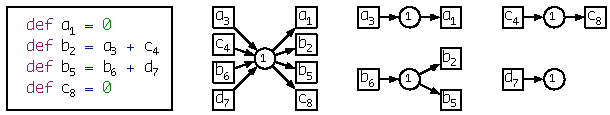
\includegraphics{figures/scope-graphs/global/example}
  \caption{%
    Program with variable declarations and references~(left), 
    corresponding scope graph~(center), and resolution graphs~(right).}
  \figurelabel{global}
\end{center}
\end{figure}

Depending on their syntactical position,
  instances have different roles in name binding.
A \emph{binding instance} introduces a new binding for the identifier in a certain scope.
In scope graphs, a directed edge \inlinegraphics{figures/scope-graphs/legend/definition} 
  connects a scope \inlinegraphics{figures/scope-graphs/legend/scope} 
  with a binding instance \inlinegraphics{figures/scope-graphs/legend/identifier} of that scope.
A \emph{referring instance} refers to a, potentially non-existing, binding instance of the same name in a certain scope.
If such a binding instance exists, the referring instance is a \emph{bound instance},
  otherwise it is a \emph{free instance}.
In scope graphs, a directed edge \inlinegraphics{figures/scope-graphs/legend/reference} 
  connects a referring instance \inlinegraphics{figures/scope-graphs/legend/identifier} 
  to its scope \inlinegraphics{figures/scope-graphs/legend/scope}.
In the example from \Figure{global},   
  all instances occur in the global scope \inlinegraphics{figures/scope-graphs/global/scopes} of the program
  which has incoming edges from referring instances \inlinegraphics{figures/scope-graphs/global/referring}
  and outgoing edges to its binding instances \inlinegraphics{figures/scope-graphs/global/binding}.
  
% \paragraph{Local resolution}
% 
% With scope graphs, name resolution corresponds to 
%   finding \emph{resolution paths} from referring instances to binding instances of the same name.
% In the scope graph from \Figure{global},
%   we cannot find a resolution path for \inlinegraphics{figures/scope-graphs/global/referring-c}.
% Thus, this instance is a free instance. 
% In contrast, 
%   we can find resolution paths to resolve 
%   \inlinegraphics{figures/scope-graphs/global/referring-a} and
%   \inlinegraphics{figures/scope-graphs/global/referring-b}, 
%   which makes those instances bound instances.
% So far, we only consider local resolution paths.



\newtheorem{definition}{Definition}
\begin{definition}[Local resolution path]
  A \emph{local resolution path for \smcode{i}} is
  a path \inlinegraphics{figures/scope-graphs/legend/local-resolution}
  from a referring instance %\inlinegraphics{figures/scope-graphs/legend/identifier} 
  to a binding instance %\inlinegraphics{figures/scope-graphs/legend/identifier} 
  of the same identifier \smcode{i}
  in the same scope \smcode{s}.
\end{definition}

%\paragraph{Local ambiguities}
%\paragraph{Local ambiguities.}

We can construct the \emph{resolution graph} of a particular instance,
  by restricting a scope graph to the nodes and edges from resolution paths of that instance.
\Figure{global} shows the resolution graphs for \inlinegraphics{figures/scope-graphs/global/referring-a} and
  \inlinegraphics{figures/scope-graphs/global/referring-b}.
Since their is only a single resolution path for \inlinegraphics{figures/scope-graphs/global/referring-a},
  its resolution graph is linear.
In contrast, the resolution graph for \inlinegraphics{figures/scope-graphs/global/referring-b} branches,
  since we can find paths to different binding instances \inlinegraphics{figures/scope-graphs/global/binding-b}.
We call such resolutions \emph{ambigous}.
In this case, the ambiguity is caused by 
  two conflicting binding instances \inlinegraphics{figures/scope-graphs/global/binding-b}
  in the same scope.
With scope graphs, we can define such conflicts in terms of paths:

\begin{definition}[Local conflict]
A binding instance \inlinegraphics{figures/scope-graphs/legend/definition} 
  \emph{conflicts locally}
  with another binding instance \inlinegraphics{figures/scope-graphs/legend/definition} 
  of the same identifier \smcode{i}
  in the same scope \smcode{s}.
\end{definition}

\paragraph{Lexical scoping}

A program typically defines several scopes.
For example, 
  the \kw{fix} and \kw{fun} expressions in the program in \Figure{lexical} 
  introduce two scopes for their argument expressions.
The corresponding scope graph in \Figure{lexical}
  represents these scopes as circle nodes 
    \inlinegraphics{figures/scope-graphs/lexical/fix-scope}
    \inlinegraphics{figures/scope-graphs/lexical/fun-scope}.
Scopes can be nested.
In scope graphs, a directed edge \inlinegraphics{figures/scope-graphs/legend/lexical} 
  connects a nested scope \inlinegraphics{figures/scope-graphs/legend/nested} 
  to its surrounding parent scope \inlinegraphics{figures/scope-graphs/legend/parent}.

\begin{figure}[htb]
\begin{center}
  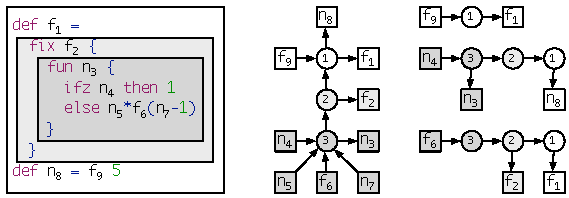
\includegraphics[trim=0.175cm 0cm 0cm 0cm]{figures/scope-graphs/lexical/example}
  \caption{%
    Lexical scopes in a function declaration~(left), 
    corresponding scope graph~(center), and resolution graphs~(right).}
  \figurelabel{lexical}
\end{center}
\end{figure}

In the example from \Figure{lexical},
  three scopes form a linear nesting hierarchy \inlinegraphics{figures/scope-graphs/lexical/nested}.
The two top-level variable declarations introduce two binding instances 
  \inlinegraphics{figures/scope-graphs/lexical/binding-f0}
  \inlinegraphics{figures/scope-graphs/lexical/binding-n0}
and a referring instance 
  \inlinegraphics{figures/scope-graphs/lexical/referring-f0}
in global scope \inlinegraphics{figures/scope-graphs/lexical/global-scope}.
The \kw{fix} expression introduces another binding instance 
  \inlinegraphics{figures/scope-graphs/lexical/binding-f1}
  in a new scope \inlinegraphics{figures/scope-graphs/lexical/fix-scope}
  which is nested in the global scope \inlinegraphics{figures/scope-graphs/lexical/global-scope}.
Finally, the \kw{fun} expression introduces another binding instance
  \inlinegraphics{figures/scope-graphs/lexical/binding-n2}
  and four referring instances 
  \inlinegraphics{figures/scope-graphs/lexical/referring-n2}
  \inlinegraphics{figures/scope-graphs/lexical/referring-f2}
  in a new scope \inlinegraphics{figures/scope-graphs/lexical/fun-scope}
  which is nested in the scope \inlinegraphics{figures/scope-graphs/lexical/fix-scope} of the fix expression.
 

%\paragraph{Lexical resolution}

A referring instance can be resolved either in its local scope or
  in one of its surrounding parent scopes.
Thus, we need to extend Definition~1 to allow chains of nested scopes.

\begin{definition}[Lexical resolution path]
A \emph{lexical resolution path for \smcode{i}} is
  a path \inlinegraphics{figures/scope-graphs/legend/lexical-resolution}
  from a referring instance 
  to a binding instance  
  of the same identifier \smcode{i}, 
    iff \inlinegraphics{figures/scope-graphs/legend/lexical-path} is a \emph{lexical scope path}.
Thereby, a \emph{lexical scope path} is either
a (degenerated) path \inlinegraphics{figures/scope-graphs/legend/scope}, or 
a path \inlinegraphics{figures/scope-graphs/legend/lexical-induct}
  from a nested scope \inlinegraphics{figures/scope-graphs/legend/nested-induct}
  to its ancestor scope \inlinegraphics{figures/scope-graphs/legend/parent}, 
    iff \inlinegraphics{figures/scope-graphs/legend/lexical-path} is a lexical scope path.
\end{definition}

\Figure{lexical} provides the resolution graphs according to the scope graph from the same figure.
First, \inlinegraphics{figures/scope-graphs/lexical/referring-f0} can be resolved locally.
Second, \inlinegraphics{figures/scope-graphs/lexical/referring-n2} can be resolved 
  either locally to \inlinegraphics{figures/scope-graphs/lexical/binding-n2} 
  or to \inlinegraphics{figures/scope-graphs/lexical/binding-n0} in the outermost surrounding scope.
Finally, \inlinegraphics{figures/scope-graphs/lexical/referring-f2} cannot be resolved locally but to
  \inlinegraphics{figures/scope-graphs/lexical/binding-f1} and
  \inlinegraphics{figures/scope-graphs/lexical/binding-f0} in its two surrounding scopes.


%\paragraph{Lexical ambiguities}

Hierarchies of nested lexical scopes introduce another source for ambiguous resolutions.
A referring instance can not only be resolved to conflicting binding instances in the same scope,
but also to conflicting binding instances in different scopes in the scope hierarchy.
Both ambiguities in the example from \Figure{lexical} are caused by the latter.
In the case of \inlinegraphics{figures/scope-graphs/lexical/referring-n2},
  the local binding instance \inlinegraphics{figures/scope-graphs/lexical/binding-n2}
  conflicts with \inlinegraphics{figures/scope-graphs/lexical/binding-n0}
  from the global scope.
In the case of \inlinegraphics{figures/scope-graphs/lexical/referring-f2},
  no local binding instance is involved.
  Instead, the conflict arises in the parent scope,
  where
    \inlinegraphics{figures/scope-graphs/lexical/binding-f1}
    conflicts with \inlinegraphics{figures/scope-graphs/lexical/binding-f0}
    from the global scope.

Such conflicts are typically resolved in favour of binding instances
  in scopes closer to the referring instances.
Binding instances in a nested scope \emph{shadow} 
  binding instances of the same name from surrounding scopes.
Similar to local conflicts, we can define shadowing in terms of paths in a scope graph.

\begin{definition}[Lexical shadowing]
A binding instance \inlinegraphics{figures/scope-graphs/legend/shadowing}
  \emph{shadows} 
  another binding instance \inlinegraphics{figures/scope-graphs/legend/shadowed} 
    of the same identifier \smcode{i}
  \emph{in scope \smcode{sn}},
  iff there exist a lexical scope path \inlinegraphics{figures/scope-graphs/legend/lexical-path}.
\end{definition}

With shadowing, name resolution corresponds to 
  finding paths from referring instances to unshadowed binding instances of the same name.
The ambiguities in the example from \Figure{lexical} are
  resolved in favour of the more local binding instances 
    \inlinegraphics{figures/scope-graphs/lexical/binding-n2} and
    \inlinegraphics{figures/scope-graphs/lexical/binding-f1}.

\paragraph{Alternative lexical scope hierarchies}

Similar syntactic structures can introduce different lexical scope hierarchies.
For example, 
  the programs in \Figure{let} employ different kinds of \kw{let} expressions,
    resulting in different scoping hierarchies for syntactically equivalent binding parts.
The \kw{letpar} expression introduces only a single scope \inlinegraphics{figures/scope-graphs/lets/body-scope} 
  for the body of the expression.
Binding instances \inlinegraphics{figures/scope-graphs/lets/par-bind} 
  from the binding parts are connected to the new scope.
As a consequence, referring instances \inlinegraphics{figures/scope-graphs/lets/par-bind-refer} 
  from the binding parts resolve to binding instances \inlinegraphics{figures/scope-graphs/lets/global-bind} 
  in the global scope.

\begin{figure}[htb]
\begin{center}
  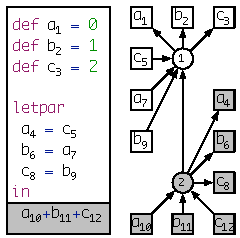
\includegraphics[trim=0.7cm 0cm 0cm 0cm]{figures/scope-graphs/lets/par}
  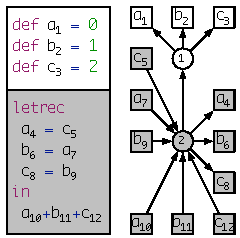
\includegraphics[trim=0.7cm 0cm 0cm 0cm]{figures/scope-graphs/lets/rec}
  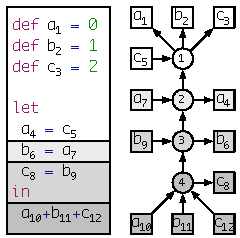
\includegraphics{figures/scope-graphs/lets/seq}
  \caption{Different kinds of let expressions and corresponding lexical scope hierarchies.}
  \figurelabel{let}
\end{center}
\end{figure}

The \kw{letrec} expression also introduces a single scope \inlinegraphics{figures/scope-graphs/lets/body-scope},
  but includes the binding parts in this scope.
This way, referring instances \inlinegraphics{figures/scope-graphs/lets/rec-bind-refer}
  from the binding parts now resolve to binding instances \inlinegraphics{figures/scope-graphs/lets/par-bind}
  from the binding parts.
Together with a disambiguation strategy which prefers local bindings, 
  binding parts can shadow other bindings in the whole \kw{letrec} expression.
Finally, the sequential \kw{let} expression introduces nested scopes \inlinegraphics{figures/scope-graphs/lets/scopes} 
  for each binding part.
These scopes include subsequent binding parts and the body of the \kw{let} expression.
In contrast to \kw{letrec} expressions,
  the same \kw{let} expression can bind instances of the same identifier multiple times,
  where new bindings shadow previous bindings.
Though, binding parts in \kw{let} expressions can only shadow bindings in subsequent binding parts and in the body,
  while binding parts in \kw{letrec} expressions can shadow bindings in preceding binding parts as well.
Hence, \inlinegraphics{figures/scope-graphs/lets/c2} resolves to \inlinegraphics{figures/scope-graphs/lets/c1}
  in global scope and not to \inlinegraphics{figures/scope-graphs/lets/c3} in a subsequent binding part.
  

% \begin{figure}[htb]
% \begin{center}
%   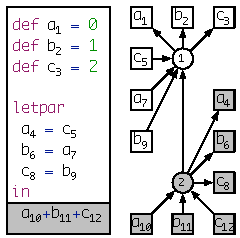
\includegraphics[trim=0.7cm 0cm 0cm 0cm]{figures/scope-graphs/lets/par}
%   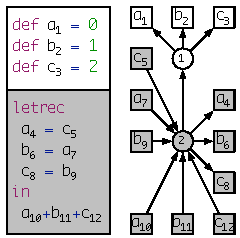
\includegraphics[trim=0.7cm 0cm 0cm 0cm]{figures/scope-graphs/lets/rec}
%   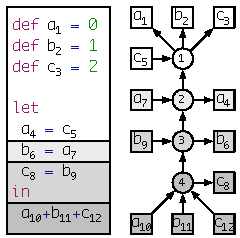
\includegraphics{figures/scope-graphs/lets/seq}
%   \caption{Scoping in different kinds of let expressions.}
%   \figurelabel{let}
% \end{center}
% \end{figure}

\paragraph{Named scopes and qualified names}

Language constructs might associate names with corresponding scopes.
For example, each module in the program in \Figure{qualified}
  associates a module name with the scope of the module, 
    which captures the declarations of the module.
We call such scopes \emph{named scopes}.
Binding instances in named scopes can be accessed from other scopes via the name of the scope.
For example, the program in \Figure{qualified} uses \emph{qualified names} to access declarations of a module from another module.

We introduce a second kind of edges, to model named scopes and qualified names.
A directed edge \inlinegraphics{figures/scope-graphs/legend/named} connects 
  a binding instance \inlinegraphics{figures/scope-graphs/legend/identifier} 
  to its associated named scope \inlinegraphics{figures/scope-graphs/legend/scope}.
A complementary directed edge \inlinegraphics{figures/scope-graphs/legend/qualified} connects 
  a qualified referring instance \inlinegraphics{figures/scope-graphs/legend/identifier} 
  to a qualifying referring instance \inlinegraphics{figures/scope-graphs/legend/qualifier}.
  
With qualified names, we can resolve to binding instances in a named scope, 
  even if these instances are not in the lexical scope of the referring instance.
In the example program in \Figure{qualified}, \inlinegraphics{figures/scope-graphs/qualified/b2} resolves to
  \inlinegraphics{figures/scope-graphs/qualified/b1}, which is not in the lexical scope of module \smcode{C}.
The corresponding resolution path includes the resolution path of the qualifier, 
  which is surrounded by two \inlinegraphics{figures/scope-graphs/legend/edge2} edges.
The opening edge  \inlinegraphics{figures/scope-graphs/qualified/opening} 
  is provided by the qualified name, 
  while the closing edge \inlinegraphics{figures/scope-graphs/qualified/closing} 
  is provided by a named scope.
The resolution path is completed by the binding instance \inlinegraphics{figures/scope-graphs/qualified/finish}.
%
The resolution of \inlinegraphics{figures/scope-graphs/qualified/b3} illustrates resolution of nested qualifiers.
In general, each nested qualifier needs to be resolved in the named scope of its preceeding qualifier, 
  before we can resolve the qualified name in the named scope of the last qualifier.
  
\begin{figure}[t]
\begin{center}
  %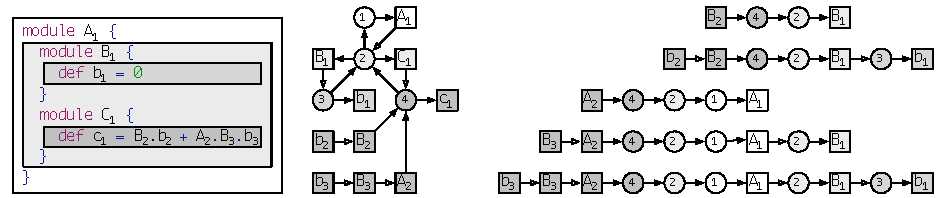
\includegraphics[trim=0.175cm 0cm 0cm 0cm]{figures/scope-graphs/qualified/example}
  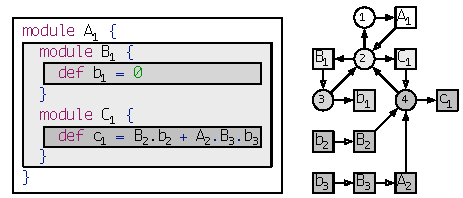
\includegraphics[trim=0.175cm 0cm 0cm 0cm]{figures/scope-graphs/qualified/example2}
  \vspace{0.35cm}
  
  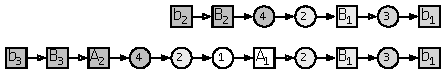
\includegraphics{figures/scope-graphs/qualified/resolution2}
  \caption{Named module scopes and qualified name access~(left), corresponding scope graph~(right) and resolution graphs~(bottom).}
  \figurelabel{qualified}
\end{center}
\end{figure}


\begin{definition}[Qualified resolution path]
  A path \inlinegraphics{figures/scope-graphs/legend/qualified-resolution}
  from a referring instance \inlinegraphics{figures/scope-graphs/legend/identifier} 
  to a binding instance \inlinegraphics{figures/scope-graphs/legend/identifier} of the same name
  is a \emph{qualified resolution path for \smcode{i}}, 
    iff \inlinegraphics{figures/scope-graphs/legend/qualifier-resolution} is 
      a lexical or qualified resolution path for \emph{\smcode{q}}.
\end{definition}

\paragraph{Imports}

Import directives introduce binding instances from a named scope into another scope.
In scope graphs, a directed edge \inlinegraphics{figures/scope-graphs/legend/import} connects 
  an importing scope \inlinegraphics{figures/scope-graphs/legend/scope}
  with a reference \inlinegraphics{figures/scope-graphs/legend/identifier} to the imported scope.
During resolution, these edges enable scope paths from importing scopes to imported scopes,
  making binding instances in the imported scope reachable for the importing scope.
This is orthogonal to lexical scoping, where scope paths from nested scopes to surrounding scopes
  make binding instances available to the nested scopes.  
Though, lexical scoping and importing cannot be combined arbitrarily.
While resolution should consider imports in surrounding scopes,
  it should not consider surrounding scopes of imported scopes.
This leads to the following definition of resolution paths:

\begin{definition}[Resolution path]
A \emph{resolution path for \smcode{i}} is either
  a path \inlinegraphics{figures/scope-graphs/legend/lexical-resolution}, 
    iff \inlinegraphics{figures/scope-graphs/legend/lexical-path} is a \emph{scope path}, or
  a path \inlinegraphics{figures/scope-graphs/legend/qualified-resolution},
    iff \inlinegraphics{figures/scope-graphs/legend/qualifier-resolution} is a resolution path for \emph{\smcode{q}}.

Thereby, a \emph{scope path} is either
  a (degenerated) path \inlinegraphics{figures/scope-graphs/legend/scope}, or 
  a path \inlinegraphics{figures/scope-graphs/legend/lexical-induct}, 
    iff \inlinegraphics{figures/scope-graphs/legend/lexical-path} is a scope path, or
  a path \inlinegraphics{figures/scope-graphs/legend/import-induct}, 
    iff \inlinegraphics{figures/scope-graphs/legend/lexical-path} is a scope path and
    \inlinegraphics{figures/scope-graphs/legend/import-resolution} is a resolution path for \emph{\smcode{j}}.
\end{definition}

\Figure{includes} shows an example program with three modules.
To resolve \inlinegraphics{figures/scope-graphs/imports/vb1} in \inlinegraphics{figures/scope-graphs/imports/s2},
  we need to consider the import of \inlinegraphics{figures/scope-graphs/imports/B1},
  which resolves to \inlinegraphics{figures/scope-graphs/imports/B2}.
In its associated scope \inlinegraphics{figures/scope-graphs/imports/s3},
  we find \inlinegraphics{figures/scope-graphs/imports/vb2} 
  and another import \inlinegraphics{figures/scope-graphs/imports/C1},
  which resolves to \inlinegraphics{figures/scope-graphs/imports/C2}.
In its associated scope \inlinegraphics{figures/scope-graphs/imports/s4}, 
  we find \inlinegraphics{figures/scope-graphs/imports/vb3}. 
%   
This ambigous resolution is caused by a conflict between 
  the local binding instance \inlinegraphics{figures/scope-graphs/imports/vb2}
  and the imported binding instance \inlinegraphics{figures/scope-graphs/imports/vb3}.
In general, a conflict occurs, 
if two local or imported binding instances have the same name.

\begin{definition}[Conflict]
A binding instance \inlinegraphics{figures/scope-graphs/legend/conflict1}
  \emph{conflicts in scope} \inlinegraphics{figures/scope-graphs/legend/scope}  with 
  another binding instance \inlinegraphics{figures/scope-graphs/legend/conflict2} of the same name,
  iff there exist local scope paths 
    \inlinegraphics{figures/scope-graphs/legend/conflict3} and
    \inlinegraphics{figures/scope-graphs/legend/conflict-4}.

\noindent Thereby, a \emph{local scope path} is either
  a (degenerated) path \inlinegraphics{figures/scope-graphs/legend/scope}, or 
  a path \inlinegraphics{figures/scope-graphs/legend/import-induct}, 
    iff \inlinegraphics{figures/scope-graphs/legend/lexical-path} is a local scope path and
    \inlinegraphics{figures/scope-graphs/legend/import-resolution} is a resolution path for \emph{\smcode{j}}.
\end{definition}

\begin{figure}[t]
\begin{center}
  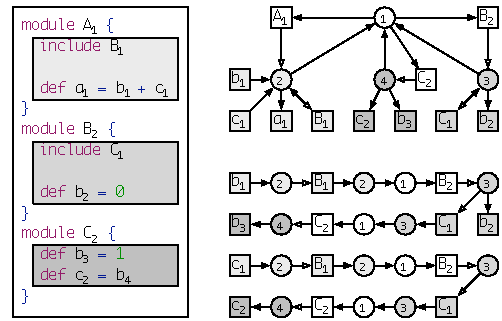
\includegraphics[trim=0.175cm 0cm 0cm 0cm]{figures/scope-graphs/imports/include}
  \caption{Includes of modules.}
  \figurelabel{includes}
  \bigskip
  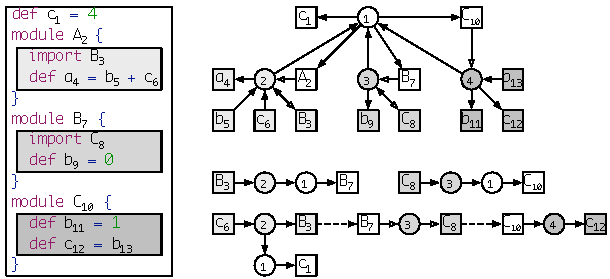
\includegraphics[trim=0.175cm 0cm 0cm 0cm]{figures/scope-graphs/imports/imports}
  \caption{Imports of modules.}
  \figurelabel{imports}
\end{center}
\end{figure}

\paragraph{Alternative import scope hierarchies}

Earlier in this section, we showed that similar syntactic constructs might yield different lexical scope hierarchies.
This also holds for import scope hierarchies.
For example, the program in \Figure{imports} is a variant of the previous program from \Figure{includes},
  where local declarations can hide imported declarations and local imports hide transitive imports.
Each module now introduces two nested scopes.
Import edges connect only to the outer scope.
This way, local declarations can hide imported declarations.
For example, 
  the resolution of \inlinegraphics{figures/scope-graphs/imports/vb1} in \Figure{imports} 
  does no longer has a conflict between a local declaration and an imported declaration.
Though, the resolution is still ambigous.
The ambiguity is caused by module names which are now associated with two scopes.
This is needed to still allow for transitive imports, 
  where both local declarations and imported declarations can be imported.
The ambiguity can be resolved by an explicit order of scopes associated with names.
In the case of \kw{import} directives, we want to prefer the inner scope of a module (for local definitions) 
  over its outer scope (for imports).

% \begin{definition}[Shadowing]
% A binding instance \inlinegraphics{figures/scope-graphs/legend/identifier}
%   \emph{shadows} another binding instance \inlinegraphics{figures/scope-graphs/legend/shadowed} of the same name
%   \emph{in scope \smcode{sn}},
%   iff there exist a local scope path \ldots 
%   and a scope path \inlinegraphics{figures/scope-graphs/legend/lexical-path}.
% \end{definition}

	\newpage\clearpage
	\section{A Theory of Visibility}

naming conflict: multiple resolution paths for same identifier

some naming conflicts are resolved by policies for visibility 

thesis: shadowing / visibility is independent / orthogonal to resolution paths

systematic analysis of the design space of shadowing as expressed in terms of path well-formedness and specificity ordering
\begin{itemize}
 \item  model different kinds of imports through flags on imports
\item transitive vs non-transitive vs non-transitive+export
\item include vs import vs prefer-imported: maybe use a precedence value in the imports
\item imports with inherited lexical scope (handled by well-formedness)
\end{itemize}

Add flags to imports to describe the different policies, should be handled by well-formedness of the resolution path

\newcommand{\flag}[1]{\overline{#1}}

\paragraph{Import Policies}
To reflect the different imports policies, we add boolean flags to the imports,
when no flag is specified the default behavior is used.
Assume some \emph{import B} is declared in a module {\it A},
\begin{itemize}
 \item If the Import/Export flag $e$ of this import is $0$ then the definition in {\it B} are visible in $A$ and if it is $1$ the definitions
  in {\it B} are also visible from every scope importing \emph{A}.
 \item If the transitivity flag $t$ is $0$ then the resolution can only use the definitions or exports of the imported module else
  the resolution can use all the import clauses in the imported scopes
 \item If the parent (recursive) flag $r$ is $0$ then the resolution process can only continue through possible imports else it 
  can also look into the parent scope
\end{itemize}
The flag of an import is thus a triple of booleans and denoted $\flag{etr}$, for example a non-transitive export that do not allow recursive call
to parent has flag $\flag{100}$.


% The precedence flag $pr^{F}$ can be either set to:
%   \begin{itemize}
%    \item Usual import $u$ whose precedence is lower than the definition, thus a resolution using directly a definition is preferred
%     over an usual import
%    \item Include import $i$ whose precedence is the same than a definition
%    \item Pref import $p$ whose precedence is higher than a definition, such an import is preferred over a direct definition
%   \end{itemize}

??? what if we want priority of import over parents ? for example import with same precedence as parent, parent preferred over imports ??? 
Back to the idea of giving a precedence to imports in algorithm: try to resolve with precedence n, if you find something then done else try with
prec (n+1), parent and definition are only one of these way.

Automata in Figure \ref{fig:algoterm} for the correctness of the path, the states corresponds to different authorization first component is the transitivity flag, i.e. are you allowed to 
use simple imports, second component is the parent flag, i.e. can you look inside the parent scope. Transitions are either parent rule $P$, or imports flags 

\begin{figure}
\centering
\begin{tikzpicture}[shorten >=1pt,auto]

\tikzset{>=stealth',
    every edge/.append style={->}
  }
      \node[circle,draw] (TR) at (0,2.6) {\it 11};
      \node[circle,draw] (TX) at (4.5,5.2) {\it 10};
      \node[circle,draw] (NX) at (3,2.6) {\it 00};
      \node[circle,draw] (NR) at (4.5,0) {\it 01};
      \node (ri) at (4.5,2) {};
      
     \path 

     (TR) edge[loop left] node[left] {\small $\flag{x11} + P$} (TR)
     (TR.90) edge[bend left=35] node[above left] {\small $\flag{x10}$} (TX.175)
     (TR) edge[bend left=10] node[above] {\small $\flag{x00}$} (NX)
     (TR.280) edge[bend right=35] node[above right] {\small $\flag{x01}$} (NR.175)

     (TX) edge[loop above] node[above] {\small $\flag{x10}$} (TX)
          edge[bend left=10] node[right] {\small $\flag{x00}$} (NX)
     (TX.185) edge[bend right=35] node[below right] {\small $\flag{x11}$} (TR.80)
     (TX.340) edge[bend left=50] node[right] {\small $\flag{x01}$} (NR.20)

     (NX) edge[loop right] node[right] {\small $\flag{100}$} (NX)
          edge[bend left=10] node[left] {\small $\flag{110}$} (TX)
          edge[bend left=10] node[right] {\small $\flag{101}$} (NR)
     (NX) edge[bend left=10]  node[below] {\small $\flag{111}$} (TR)

     (NR) edge[loop below] node[below] {\small $\flag{101} + P$} (NR)
     (NR.30) edge[bend right=50] node[left] {\small $\flag{110}$} (TX.330)
     (NR) edge[bend left=10] node[left] {\small $\flag{100}$} (NX)
     (NR.185) edge[bend left=35] node[below left] {\small $\flag{111}$} (TR.270);

\end{tikzpicture}
%\rule{\textwidth}{.1pt}
\caption{Path Well Formedness Automata}
\label{fig:algoterm}
\end{figure}


\begin{figure}
\begin{boxedminipage}{\hsize}

\textbf{Edges in scope graph}

\smallskip

	\infrule{R}{
		x^p \in \R{S}
	}{
		\mathcal{I} \vdash x^p \scopea{x}{R(x^p)} S
	}
	
\smallskip

	\infrule{D}{
		d_x \in \D{S}
	}{
		\mathcal{I} \vdash S \scopea{x}{D(d_x)} d_x
  }

\smallskip

% 	\infrule{T}{}{
% 		\mathcal{I} \vdash S_1\cdot S_2\cdot S^* \scopea{x}{T} S_2 \cdot S^*
% 	}

% \smallskip

	\infrule{Par}{
		\P{S} = S'
	}{
		\mathcal{I} \vdash S \scopea{x}{Par} S'
	}

\smallskip

	\infrule{I}{
		y^p \in \mathcal{I}(S_1)  
		\tab 
		y^p \notin \mathcal{I} 
		\tab
		y^p\!,\mathcal{I} \vdash y^p \resolvea{P^*}\!\!\!d_y^{S_2}		
	}{
		\mathcal{I} \vdash S_1 \scopea{x}{I^t(y^p,P^*)} S_2 
	}

\smallskip

% 	\infrule{I}{
% 		y^p \in \I{S_1}  
% 		\tab 
% 		y^p \notin \mathcal{I} 
% 		\tab
% 		y^p\!,\mathcal{I} \vdash y^p \resolvea{P^*}\!\!\!d_y^{S_2^*}	
% 	}{
% 		\mathcal{I} \vdash S_1\cdot S_1^* \scopea{x}{I(y^p\!,P^*)} S_2^* 
% 	}

% \smallskip

\textbf{Path composition}

	\infrule{C1}{}{
		\mathcal{I} \vdash d_x \lra{[]}{x} d_x
	}

\smallskip

	\infrule{C2}{
		\mathcal{I} \vdash A \scopea{x}{P} B
		\tab 
		\mathcal{I} \vdash B \lra{P^*}{x} C
	}{
		\mathcal{I} \vdash A \lra{P\cdot P^*}{x} C
	}

\smallskip
\textbf{Resolution}

	\infrule{Res}{
 		\begin{array}{c}
    	\mathcal{I} \vdash x^p \lra{P^*_1}{x} d_x
			\tab
			\tab
			\tab
			P^*_1 : WFP
    	\\
  		\forall d'_x,P^*_2(\mathcal{I} \vdash x^p \lra{P^*_2}{x} d'_x\Rightarrow\neg
  	P^*_2 < P^*_1)
  	\end{array}
	}{
		\mathcal{I} \vdash x^p \resolvea{P^*_1} d_x
	}

\bigskip


\end{boxedminipage}
\caption{Resolution Calculus}
\label{fig:calculus}
\end{figure}


%\begin{figure}[p]

\begin{minipage}[t]{.49\hsize}
\begin{boxedminipage}[t]{\hsize}
\textbf{References and declarations}
\begin{itemize}
  \item $\mbox{$\dsi{x}{i}{S}$}$: declaration with name $x$ at position $i$ and optional
  associated named scope $S$
  \item $\ri{x}{i}$: reference with name $x$ 
  at position~$i$ 
\end{itemize}
\textbf{Scope graph}
\begin{itemize}
  \item $\G$: scope graph
  \item $\S{\G}$: scopes $S$ in $\G$ 
  \item $\D{S}$: declarations $\dsi{x}{i}{S'}$ in $S$
  \item $\R{S}$: references $\ri{x}{i}$ in $S$
  \item $\I{S}$: imports $\ri{x}{i}$ in $S$
  \item $\P{S}$: parent scope of $S$
\end{itemize}
\textbf{Well-formedness properties}
\begin{itemize}
  \item $\P{S}$ is a partial function
  \item The parent relation is well-founded
  \item Each $\ri{x}{i}$ and $\di{x}{i}$ appears in exactly one scope $S$
\end{itemize}
\end{boxedminipage}
\caption{Scope graphs}
\figurelabel{scope-graph}
\end{minipage}
\begin{minipage}[t]{.49\hsize}
\begin{boxedminipage}[t]{\hsize}
\textbf{Resolution paths}
\vspace*{-0.4\baselineskip}
$$\begin{array}{rl}
          s & := \dstep{\di{x}{i}}\ |\ \istep{\ri{x}{i}}{\dsi{x}{j}{S}}\ |\ \pstep\\
          p & := []\ |\ s\ |\ p\cdot p\\
          & \mbox{\rm (inductively generated)} \\[0pt]
          [] \cdot p & = p \cdot [] = p\\
          (p_1 \cdot p_2) &\cdot\ p_3  = p_1 \cdot (p_2 \cdot p_3)
\end{array}$$ 

\textbf{Well-formed paths}

\vspace*{-0.5\baselineskip}

\[
	   \WF(p) \Leftrightarrow p \in \pstep^* \cdot \istep{\_}{\_}^* 
\]
	
\textbf{Specificity ordering on paths}

%\bigskip

	\infrule{DI}{}{
		\dstep{\_} < \istep{\_}{\_}
	}

\medskip

	\infrule{IP}{}{
		\istep{\_}{\_} < \pstep 
	}

\medskip

	\infrule{DP}{}{
		 \dstep{\_} < \pstep
	}

\medskip

    \infrule{Lex1}{
		s_1 < s_2
	}{ 
		s_1\cdot p_1 < s_2 \cdot p_2
	}


\medskip

	\infrule{Lex2}{
		p_1 < p_2
	}{ 
		s \cdot p_1 < s \cdot p_2
	}

\smallskip

\end{boxedminipage}
\caption{Resolution paths, well-formedness predicate, and specificity
ordering.}
\figurelabel{order}
\end{minipage}

\bigskip

\begin{boxedminipage}{\hsize}
\textbf{Edges in scope graph}
\smallskip

	\infrule{P}{
		\P{S_1} = S_2
	}{
		\seeni \vdash \pstep : S_1 \edge S_2
	}

\medskip

	\infrule{I}{
		\ri{y}{i} \in \I{S_1}\setminus\seeni  
		\tab
		\seeni \vdash p : \ri{y}{i} \resolve \dsi{y}{j}{S_2}
	}{
		\seeni \vdash \istep{\ri{y}{i}}{\dsi{y}{j}{S_2}} : S_1 \edge S_2 
	}

\medskip
\textbf{Transitive closure}

%\medskip
       
	\infrule{N}{
		}{
		\seeni \vdash [] : A \medge A
	}

\medskip

	\infrule{T}{
		\seeni \vdash s : A \edge B
		\tab 
		\seeni \vdash p : B \medge C
	}{
		\seeni \vdash s \cdot p : A \medge C
	}

\smallskip

\textbf{Reachable declarations}
\medskip

	\infrule{R}{
		\di{x}{i} \in \D{S'}
		\tab
		\seeni \vdash p : S \medge S'
		\tab 
		\WF(p)
	}{
		\seeni \vdash p \cdot \dstep{\di{x}{i}} : S \reach \di{x}{i}
	}

\medskip

\textbf{Visible declarations}
\medskip

\infrule{V}{
 	\seeni \vdash p : S \reach \di{x}{i}
			\tab
			\tab
			% tab
  		\forall j,p' (
  		   \seeni \vdash p' : S \reach \di{x}{j} \Rightarrow 
  		   \neg (p' < p)
  		)
  	}{
		\seeni \vdash {p} : S \resolve \di{x}{i}
	}

\medskip

\textbf{Reference resolution}

\medskip 

\infrule{X}{
		\ri{x}{i} \in \R{S}
    \tab
    \{ \ri{x}{i} \} \cup \seeni \vdash p : S \resolve \di{x}{j}
	}{
		\seeni \vdash p : \ri{x}{i} \resolve \di{x}{j}
	}
\end{boxedminipage}
\caption{Resolution calculus}
\figurelabel{rescalc}



\end{figure}




Set of \emph{seen-imports} : 
\begin{itemize}
 \item how do we introduce it ?
 \item in which cases is it really necessary ?
\end{itemize}

%%% Local Variables: 
%%% mode: latex
%%% TeX-master: "../document"
%%% End: 

	\newpage\clearpage
	\section{Resolution Automata}

the calculus depends on recursive invocations

derive a (non-deterministic) resolution automaton from the calculus

$S1 \rightarrow_x S2 \rightarrow_x S3 \rightarrow_x S4$

$S1 \rightarrow [x] S2 \rightarrow [y,x] S2 \rightarrow [y,x] S3 \rightarrow [x] S4$

formalize calculus

prove correspondence to the first calculus

- produces same paths
- apply same well-formedness \& specificity ordering

	\newpage\clearpage
	\section{Evaluation}\label{evaluation}

\begin{itemize}
\itemsep1pt\parskip0pt\parsep0pt
\item
  Coverage: can we express the name binding patterns of real languages?
\end{itemize}




%%% Local Variables: 
%%% mode: latex
%%% TeX-master: t
%%% End: 
